% =====================================================================================
% REVISIÓN 3  -  PROYECTOS DE SISTEMA INFORMÁTICO
% =====================================================================================

\section{Desarrollo del sistema} \label{sec:desarrollo_sistema} % audit:req=desarrollo_sistema

\begin{guia}[Guía: Desarrollo del sistema (Revisión 3, proyectos de sistema)]
\textbf{¿Para qué sirve?} Documenta cómo se construyó la solución: arquitectura, diseño y resultado final. Debe permitir
que otra persona entienda el sistema y pueda darle mantenimiento.

\textbf{En el texto propio de este capítulo (antes de las subsecciones) responde:}
\begin{itemize}[nosep,leftmargin=*]
  \item ¿Cuál es la arquitectura del sistema (capas, cliente-servidor, microservicios, nube)? Incluye un diagrama.
  \item ¿Qué tecnologías, versiones y librerías se usaron y para qué?
  \item ¿Cómo está organizado el código (módulos, carpetas, patrones)? Muestra solo fragmentos relevantes y explícalos.
  \item ¿Qué pruebas se hicieron (funcionales, de integración, de usabilidad) y con qué resultado?
  \item ¿Cómo se despliega o instala? ¿dónde está el repositorio?
  \item ¿Qué problemas técnicos surgieron y cómo se resolvieron?
\end{itemize}

\textbf{Extensión mínima:} 300 palabras de texto propio de este capítulo, además de las subsecciones que siguen.

\textbf{Reglas para todas las figuras:} cada diagrama o captura lleva \verb|\caption|, \verb|\label|, se cita en el texto con
\verb|Figura~\ref{fig:...}| (nunca escribas ``Figura 3'' a mano) y debe ser legible al imprimirse.

\textbf{Cómo se revisa:} coherencia con la propuesta y los requisitos, suficiencia técnica y que las subsecciones
obligatorias estén completas.
\end{guia}

El sistema se implementó como una aplicación web cliente-servidor para consultar documentación técnica de planta. El
cliente se ejecuta en el navegador y presenta la conversación, las fuentes, el historial de chats y la biblioteca de
documentos. El servidor expone una API REST con FastAPI; recibe la pregunta, valida el contrato JSON, solicita los
fragmentos pertinentes al recuperador y coordina la respuesta del agente. Esta separación permite probar cada componente
por separado y mantiene la clave del proveedor de IA fuera del navegador.

La arquitectura implementada tiene cuatro responsabilidades. El frontend contiene la interacción y el estado visual;
el backend contiene las rutas HTTP, el historial y la gestión de documentos; el agente organiza los estados de
recuperación, decisión y generación; y el índice local consulta los fragmentos preparados por el Integrante 1. La
Figura~\ref{fig:arquitectura_desarrollo} resume esta comunicación. En la versión evaluada, el índice local conserva los
metadatos de cada fragmento y deja preparado el contrato para conectarse posteriormente con PostgreSQL y pgvector.

El código se organiza en carpetas con responsabilidades separadas: \texttt{frontend/} contiene \texttt{index.html},
\texttt{css/} y \texttt{js/app.js}; \texttt{backend/main.py} expone las rutas; \texttt{backend/agent.py} define el grafo
del agente; \texttt{backend/retrieval.py} realiza la búsqueda; \texttt{backend/services/history.py} persiste las
conversaciones; y \texttt{data/} contiene documentos, fragmentos e historial de prueba. La interfaz utiliza HTML, CSS y
JavaScript sin un framework adicional, mientras que el backend usa Python, FastAPI 0.141.1 y Uvicorn 0.52.4. El flujo
del agente utiliza LangGraph 1.2.11 y plantillas de LangChain 1.4.0; el modelo configurado para esta entrega es Gemini
3.5 Flash Lite con temperatura 0.1 y un tiempo de espera de 60 segundos, como se registró en la propuesta
\cite{fastapiDocs,langchainDocs,langgraphDocs,googleGeminiApi}.

Las pruebas realizadas fueron funcionales y de integración. Primero, \texttt{GET /health} devolvió estado 200 y confirmó
que FastAPI estaba disponible. Después, el frontend cargó desde Vite y envió una pregunta al endpoint \texttt{POST /chat}.
La respuesta recuperó información sobre la prensa PH-100, mostró fuentes documentales y conservó el chat en el historial.
También se verificó \texttt{GET /documents}, que presentó seis archivos de prueba, y la navegación entre Inicio, Historial y
Documentos. Finalmente, se probó una consulta fuera del corpus, para la que el agente debe comunicar que no tiene
información suficiente. Estas pruebas no sustituyen la evaluación formal de métricas, pero comprueban la integración
entre navegador, API, recuperador, persistencia y proveedor externo.

El despliegue de prueba se realiza de forma local con el entorno virtual de Python y el servidor de desarrollo de Vite.
El repositorio de la tesina se encuentra en \url{https://github.com/ezequiel-proyectos/Plantilla-Tesina-ITI}; el código del
prototipo se conserva en la carpeta del proyecto de estadía. Entre los problemas técnicos resueltos estuvieron la
configuración de CORS para separar los puertos 5173 y 8000, la persistencia del título del chat a partir de la primera
pregunta, la apertura de fuentes mediante rutas seguras y el ajuste del scroll para que solo el recuadro de conversación
se desplace. La limitación actual es que la biblioteca local todavía depende de los fragmentos disponibles y la
persistencia vectorial queda como una integración posterior.

\begin{figure}[H]
\centering
\resizebox{\textwidth}{!}{%
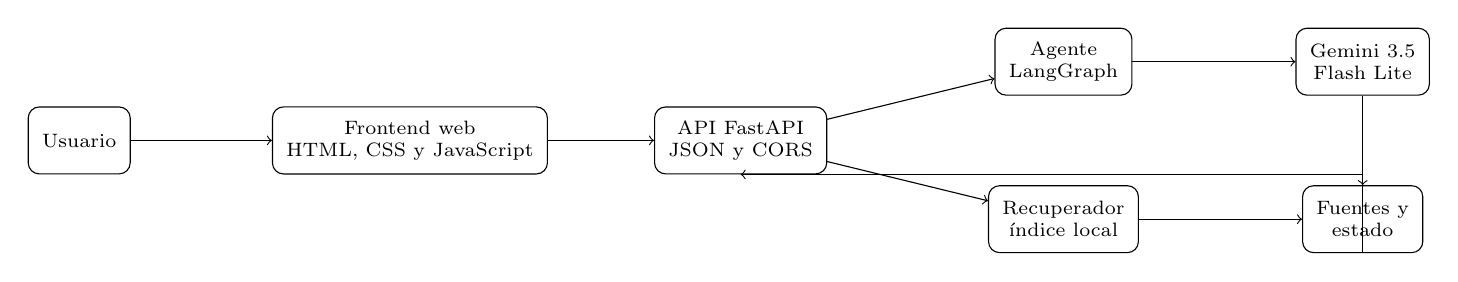
\begin{tikzpicture}[font=\scriptsize, every node/.style={draw, rounded corners, align=center, minimum height=0.85cm, inner sep=5pt}]
  \node (user) at (0,0) {Usuario};
  \node (front) at (4.2,0) {Frontend web\\HTML, CSS y JavaScript};
  \node (api) at (8.4,0) {API FastAPI\\JSON y CORS};
  \node (agent) at (12.5,1.0) {Agente\\LangGraph};
  \node (retrieval) at (12.5,-1.0) {Recuperador\\índice local};
  \node (model) at (16.3,1.0) {Gemini 3.5\\Flash Lite};
  \node (sources) at (16.3,-1.0) {Fuentes y\\estado};
  \draw[->] (user) -- (front);
  \draw[->] (front) -- (api);
  \draw[->] (api) -- (agent);
  \draw[->] (api) -- (retrieval);
  \draw[->] (agent) -- (model);
  \draw[->] (retrieval) -- (sources);
  \draw[->] (model) -- (sources);
  \draw[->] (sources.south) |- (api.south);
\end{tikzpicture}}
\caption{Arquitectura implementada del sistema web.}
\label{fig:arquitectura_desarrollo}
\end{figure}

La arquitectura de la Figura~\ref{fig:arquitectura_desarrollo} mantiene separado el canal de interacción, la lógica del
agente y la fuente documental. Esto facilita sustituir el proveedor de generación o el índice sin cambiar el contrato de
la interfaz.

\subsection{Diagramas de casos de uso} \label{sec:casos_uso} % audit:req=casos_uso

\begin{guia}[Guía: Diagramas de casos de uso]
\textbf{Debe incluir:} un diagrama general con los actores y casos de uso (relaciones \emph{include} y \emph{extend} cuando
apliquen) y la \textbf{especificación} de los casos de uso principales en una tabla (nombre, actor, precondición, flujo
normal, flujos alternos, postcondición).

\textbf{Debe responder:} ¿quiénes usan el sistema? ¿qué puede hacer cada actor? ¿cada caso de uso corresponde a un
requisito y a un objetivo específico?

\textbf{Mínimo:} 1 diagrama (figura) con explicación. Herramientas: draw.io, StarUML, PlantUML, Visual Paradigm.
\end{guia}

El actor principal es el usuario que consulta procedimientos, revisa fuentes y continúa conversaciones. El responsable de
documentación cumple un segundo rol: administra la biblioteca local y verifica que los documentos estén disponibles para
la preparación del corpus. La Figura~\ref{fig:casos_uso} relaciona ambos actores con las funciones observadas en el
frontend. La consulta incluye la recuperación de fragmentos y la generación de respuesta; cuando no existe contexto
suficiente, se extiende hacia una respuesta de incertidumbre.

\begin{figure}[H]
\centering
\resizebox{\textwidth}{!}{%
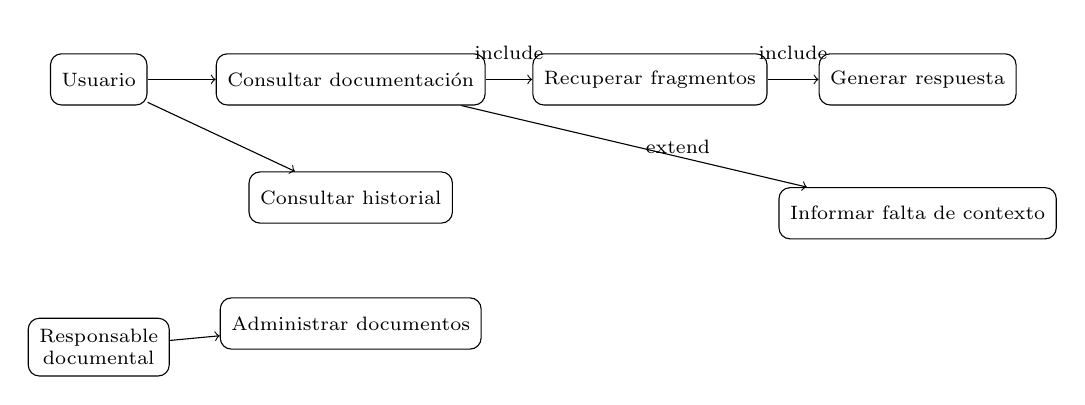
\begin{tikzpicture}[font=\scriptsize, every node/.style={draw, rounded corners, align=center, minimum height=0.65cm, inner sep=4pt}]
  \node (u) at (0,1.7) {Usuario};
  \node (a) at (0,-1.7) {Responsable\\documental};
  \node (q) at (3.2,1.7) {Consultar documentación};
  \node (h) at (3.2,0.2) {Consultar historial};
  \node (d) at (3.2,-1.4) {Administrar documentos};
  \node (r) at (7.0,1.7) {Recuperar fragmentos};
  \node (g) at (10.4,1.7) {Generar respuesta};
  \node (n) at (10.4,0.0) {Informar falta de contexto};
  \draw[->] (u) -- (q);
  \draw[->] (u) -- (h);
  \draw[->] (a) -- (d);
  \draw[->] (q) -- node[draw=none, above]{include} (r);
  \draw[->] (r) -- node[draw=none, above]{include} (g);
  \draw[->] (q) -- node[draw=none, right]{extend} (n);
\end{tikzpicture}}
\caption{Casos de uso principales del copiloto documental.}
\label{fig:casos_uso}
\end{figure}

\begin{table}[H]
\centering\small
\caption{Especificación resumida de casos de uso.}
\label{tab:casos_uso}
\begin{tabular}{p{0.15\textwidth}p{0.13\textwidth}p{0.18\textwidth}p{0.30\textwidth}p{0.18\textwidth}}
\toprule
\textbf{Caso} & \textbf{Actor} & \textbf{Precondición} & \textbf{Flujo normal} & \textbf{Alterno y postcondición}\\
\midrule
Consultar documentación & Usuario & Frontend y API disponibles. & Escribe pregunta, envía, el servidor recupera fragmentos y muestra respuesta y fuentes. & Sin contexto: informa incertidumbre; con éxito: conserva el mensaje.\\
Continuar chat & Usuario & Existe un chat de la sesión. & Abre Historial, selecciona una conversación y consulta sus mensajes. & Chat inexistente: muestra error; queda disponible la conversación seleccionada.\\
Administrar documentos & Responsable & Biblioteca accesible. & Abre Documentos, consulta archivos o selecciona documentos permitidos. & Formato inválido: rechaza la carga; la lista muestra los archivos aceptados.\\
Abrir fuente & Usuario & La respuesta contiene una cita válida. & Selecciona el nombre del documento y accede a la ruta protegida. & Documento no encontrado: API devuelve 404; no se permite salir de la carpeta autorizada.\\
\bottomrule
\end{tabular}
\end{table}

La Tabla~\ref{tab:casos_uso} muestra que los casos se relacionan con los objetivos de consultar información, recuperar
fragmentos, generar respuestas trazables y mantener una biblioteca extensible. La separación de roles evita que una
persona que solo consulta pueda modificar el corpus sin pasar por el control del responsable documental.

\subsection{Diagramas de base de datos} \label{sec:diagramas_bd} % audit:req=diagrama_bd

\begin{guia}[Guía: Diagramas de base de datos]
\textbf{Debe incluir:} el diagrama entidad-relación (o el modelo relacional / de documentos) y el
\textbf{diccionario de datos} (tabla por entidad: campo, tipo, restricciones, descripción).

\textbf{Debe responder:} ¿qué entidades y relaciones hay y por qué? ¿qué gestor de base de datos se usó y por qué? ¿está
normalizado? ¿cómo se protege la información (respaldos, permisos, datos personales)?

\textbf{Mínimo:} 1 diagrama (figura) con explicación.
\end{guia}

En esta revisión se documenta el modelo lógico que usa el prototipo. Las conversaciones se guardan en un archivo JSON y el
registro lineal de consultas en JSONL; por tanto, el diagrama representa entidades y relaciones, aunque todavía no se
despliega un gestor relacional. La biblioteca de documentos y los fragmentos son fuentes separadas: un documento puede
tener muchos fragmentos y cada mensaje puede conservar varias fuentes recuperadas. Esta decisión facilita probar la
funcionalidad sin depender de un servicio externo y mantiene abierto el traslado posterior a PostgreSQL con capacidades
vectoriales.

\begin{figure}[H]
\centering
\resizebox{\textwidth}{!}{%
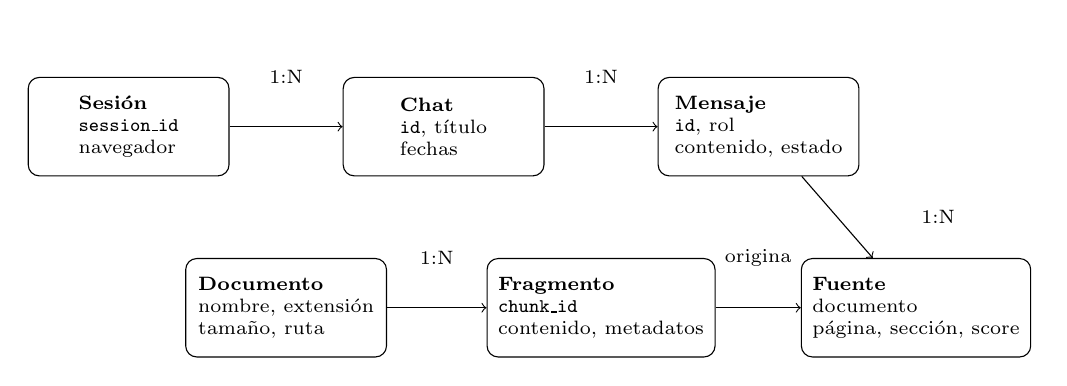
\begin{tikzpicture}[font=\scriptsize, every node/.style={draw, rounded corners, align=left, minimum width=2.55cm, minimum height=1.25cm, inner sep=4pt}]
  \node (session) at (0,2.0) {\textbf{Sesión}\\\texttt{session\_id}\\navegador};
  \node (chat) at (4.0,2.0) {\textbf{Chat}\\\texttt{id}, título\\fechas};
  \node (message) at (8.0,2.0) {\textbf{Mensaje}\\\texttt{id}, rol\\contenido, estado};
  \node (document) at (2.0,-0.3) {\textbf{Documento}\\nombre, extensión\\tamaño, ruta};
  \node (chunk) at (6.0,-0.3) {\textbf{Fragmento}\\\texttt{chunk\_id}\\contenido, metadatos};
  \node (citation) at (10.0,-0.3) {\textbf{Fuente}\\documento\\página, sección, score};
  \draw[->] (session) -- node[draw=none, above]{1:N} (chat);
  \draw[->] (chat) -- node[draw=none, above]{1:N} (message);
  \draw[->] (document) -- node[draw=none, above]{1:N} (chunk);
  \draw[->] (message) -- node[draw=none, right]{1:N} (citation);
  \draw[->] (chunk) -- node[draw=none, above]{origina} (citation);
\end{tikzpicture}}
\caption{Modelo lógico de datos para conversaciones y recuperación documental.}
\label{fig:modelo_datos}
\end{figure}

La Figura~\ref{fig:modelo_datos} distingue el historial de conversación del corpus documental. En el prototipo las
entidades se serializan en archivos locales; el control de acceso se limita a la sesión del navegador y las rutas de
documentos validan que el archivo solicitado permanezca dentro de \texttt{data/raw}. No se almacenan datos personales reales
en las pruebas. Para una instalación productiva se deberán agregar permisos, respaldos y una base de datos con índices y
restricciones formales.

\begin{longtable}{p{0.13\textwidth}p{0.18\textwidth}p{0.15\textwidth}p{0.22\textwidth}p{0.24\textwidth}}
\caption{Diccionario de datos del modelo lógico.}\label{tab:diccionario_datos}\\
\toprule
\textbf{Entidad} & \textbf{Campo} & \textbf{Tipo} & \textbf{Restricción} & \textbf{Descripción}\\
\midrule
\endfirsthead
\toprule
\textbf{Entidad} & \textbf{Campo} & \textbf{Tipo} & \textbf{Restricción} & \textbf{Descripción}\\
\midrule
\endhead
Sesión & \texttt{session\_id} & texto & identificador de sesión & Distingue el historial del navegador.\\
Chat & \texttt{id} & texto & único, requerido & Identifica una conversación.\\
Chat & \texttt{title} & texto & primera pregunta & Nombre visible en Historial.\\
Mensaje & \texttt{role} & texto & user/assistant & Indica quién produjo el mensaje.\\
Mensaje & \texttt{content} & texto & requerido & Pregunta o respuesta almacenada.\\
Documento & \texttt{name} & texto & extensión permitida & Nombre visible de la biblioteca.\\
Fragmento & \texttt{chunk\_id} & texto & único por corpus & Identificador del fragmento recuperable.\\
Fragmento & \texttt{content} & texto & requerido & Texto usado para formar el contexto.\\
Fuente & \texttt{page\_number} & entero & opcional & Página de la evidencia documental.\\
Fuente & \texttt{score} & decimal & entre 0 y 1 & Puntuación de similitud recuperada.\\
\bottomrule
\end{longtable}

\subsection{Diagramas de actividades} \label{sec:diagramas_actividades} % audit:req=diagrama_actividades

\begin{guia}[Guía: Diagramas de actividades]
\textbf{Debe incluir:} el flujo de los procesos clave del sistema (con carriles o \emph{swimlanes} por actor cuando hay
varios participantes), con inicio, decisiones, acciones y fin.

\textbf{Debe responder:} ¿cuál es el flujo de cada proceso importante? ¿qué pasa en los casos de error? ¿corresponde a
algún caso de uso?

\textbf{Mínimo:} 1 diagrama (figura) con explicación.
\end{guia}

El proceso principal corresponde al caso de uso de consulta documental. El usuario inicia la actividad al escribir una
pregunta; el frontend valida que no esté vacía y la envía como JSON. FastAPI valida el esquema, el recuperador obtiene
los fragmentos que superan el umbral y el agente decide si existe contexto suficiente. Si no lo hay, se devuelve una
respuesta de incertidumbre. Si lo hay, se consulta el modelo, se agregan citas y se conserva el turno en el historial.
Los errores de proveedor o de red terminan en un estado visible para el usuario, sin exponer la clave ni detener la
interfaz.

\begin{figure}[H]
\centering
\resizebox{0.92\textwidth}{!}{%
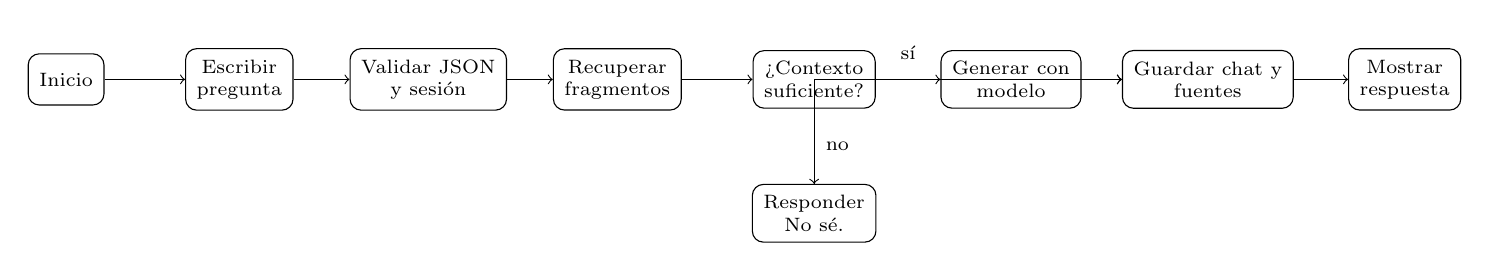
\begin{tikzpicture}[font=\scriptsize, every node/.style={draw, rounded corners, align=center, minimum height=0.65cm, inner sep=4pt}]
  \node (start) at (0,0) {Inicio};
  \node (write) at (2.2,0) {Escribir\\pregunta};
  \node (validate) at (4.6,0) {Validar JSON\\y sesión};
  \node (retrieve) at (7.0,0) {Recuperar\\fragmentos};
  \node (decide) at (9.5,0) {¿Contexto\\suficiente?};
  \node (unknown) at (9.5,-1.7) {Responder\\No sé.};
  \node (generate) at (12.0,0) {Generar con\\modelo};
  \node (save) at (14.5,0) {Guardar chat y\\fuentes};
  \node (end) at (17.0,0) {Mostrar\\respuesta};
  \draw[->] (start) -- (write);
  \draw[->] (write) -- (validate);
  \draw[->] (validate) -- (retrieve);
  \draw[->] (retrieve) -- (decide);
  \draw[->] (decide) -- node[draw=none, above]{sí} (generate);
  \draw[->] (decide) -- node[draw=none, right]{no} (unknown);
  \draw[->] (unknown) |- (save);
  \draw[->] (generate) -- (save);
  \draw[->] (save) -- (end);
\end{tikzpicture}}
\caption{Diagrama de actividades para una consulta al agente.}
\label{fig:actividad_consulta}
\end{figure}

La Figura~\ref{fig:actividad_consulta} muestra que la decisión de suficiencia ocurre antes de generar. Esta regla evita
que una pregunta fuera del corpus se convierta en una respuesta afirmativa sin evidencia. La persistencia se ejecuta
después de la respuesta para conservar tanto la pregunta como el estado, las citas y el resultado mostrado.

\subsection{Diagramas de secuencia} \label{sec:diagramas_secuencia} % audit:req=diagrama_secuencia

\begin{guia}[Guía: Diagramas de secuencia]
\textbf{Debe incluir:} la interacción entre los componentes (usuario, interfaz, servidor, base de datos, servicios
externos) para los casos de uso críticos, con los mensajes en orden temporal.

\textbf{Debe responder:} ¿qué componentes intervienen y en qué orden se comunican? ¿qué mensajes se envían y qué se
responde? ¿dónde se validan los datos?

\textbf{Mínimo:} 1 diagrama (figura) con explicación.
\end{guia}

La secuencia crítica inicia en el formulario del navegador y termina con una respuesta JSON. La validación del mensaje y
la sesión ocurre en FastAPI antes de llamar al agente. El recuperador devuelve fragmentos con \texttt{chunk\_id}, archivo,
página, sección y puntuación. Después, el agente decide si llama al modelo externo. La respuesta del modelo no se muestra
directamente: primero se combina con las citas y se guarda en el chat, lo que permite recuperar la conversación desde otra
vista del frontend.

\begin{figure}[H]
\centering
\resizebox{\textwidth}{!}{%
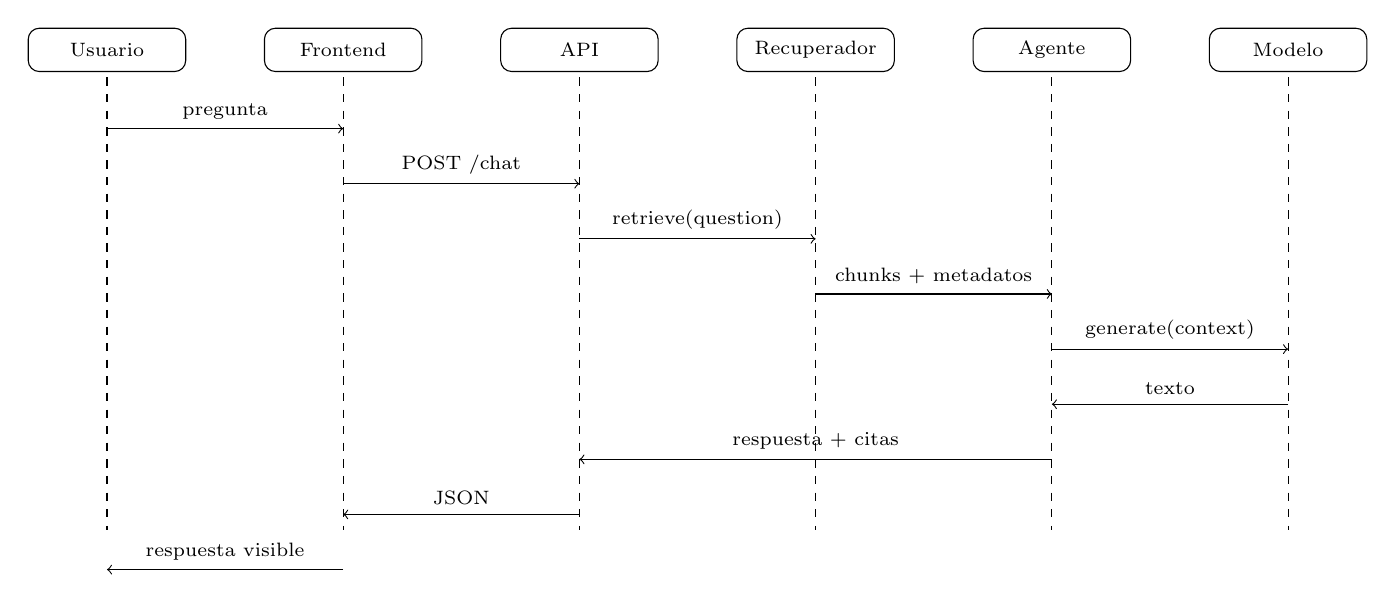
\begin{tikzpicture}[font=\scriptsize]
  \foreach \x/\name in {0/Usuario,3/Frontend,6/API,9/Recuperador,12/Agente,15/Modelo} {
    \node[draw, rounded corners, align=center, minimum width=2.0cm, minimum height=0.55cm] at (\x,0) {\name};
    \draw[dashed] (\x,-0.35) -- (\x,-6.1);
  }
  \draw[->] (0,-1) -- node[above, draw=none]{pregunta} (3,-1);
  \draw[->] (3,-1.7) -- node[above, draw=none]{POST /chat} (6,-1.7);
  \draw[->] (6,-2.4) -- node[above, draw=none]{retrieve(question)} (9,-2.4);
  \draw[->] (9,-3.1) -- node[above, draw=none]{chunks + metadatos} (12,-3.1);
  \draw[->] (12,-3.8) -- node[above, draw=none]{generate(context)} (15,-3.8);
  \draw[->] (15,-4.5) -- node[above, draw=none]{texto} (12,-4.5);
  \draw[->] (12,-5.2) -- node[above, draw=none]{respuesta + citas} (6,-5.2);
  \draw[->] (6,-5.9) -- node[above, draw=none]{JSON} (3,-5.9);
  \draw[->] (3,-6.6) -- node[above, draw=none]{respuesta visible} (0,-6.6);
\end{tikzpicture}}
\caption{Secuencia de una consulta con recuperación y generación.}
\label{fig:secuencia_consulta}
\end{figure}

La Figura~\ref{fig:secuencia_consulta} evidencia que el modelo externo no recibe la clave ni controla la sesión del
usuario. El backend es el punto que valida la entrada, determina el contexto, conserva las fuentes y construye el
contrato de salida.

\subsection{Resultado final: pantallas del sistema} \label{sec:pantallas} % audit:req=pantallas

\begin{guia}[Guía: Resultado final -- pantallas del sistema con su explicación]
\textbf{Debe incluir:} capturas de las pantallas principales del sistema funcionando, cada una con su explicación.

\textbf{Para cada pantalla responde:} ¿para qué sirve? ¿quién la usa? ¿qué casos de uso y objetivos específicos
atiende? ¿qué datos muestra o captura y cómo se valida?

\textbf{Reglas:} figuras numeradas con \verb|\caption| y \verb|\label|; sin datos personales ni confidenciales reales
(usa datos de prueba); capturas legibles. Si hay versión móvil o de escritorio, inclúyela.

\textbf{Mínimo:} 150 palabras de explicación y al menos una figura.
\end{guia}

Las capturas de esta sección se obtuvieron con la aplicación ejecutándose en el navegador y utilizando documentos de
prueba. La pantalla de inicio es el punto de entrada del usuario y contiene el formulario para enviar preguntas, además de
los accesos a historial, búsqueda y biblioteca. En la Figura~\ref{fig:pantalla_inicio} se observa el estado inicial sin
datos personales: el usuario puede escribir una consulta en el campo validado y enviarla con el botón correspondiente.

\begin{figure}[H]
\centering
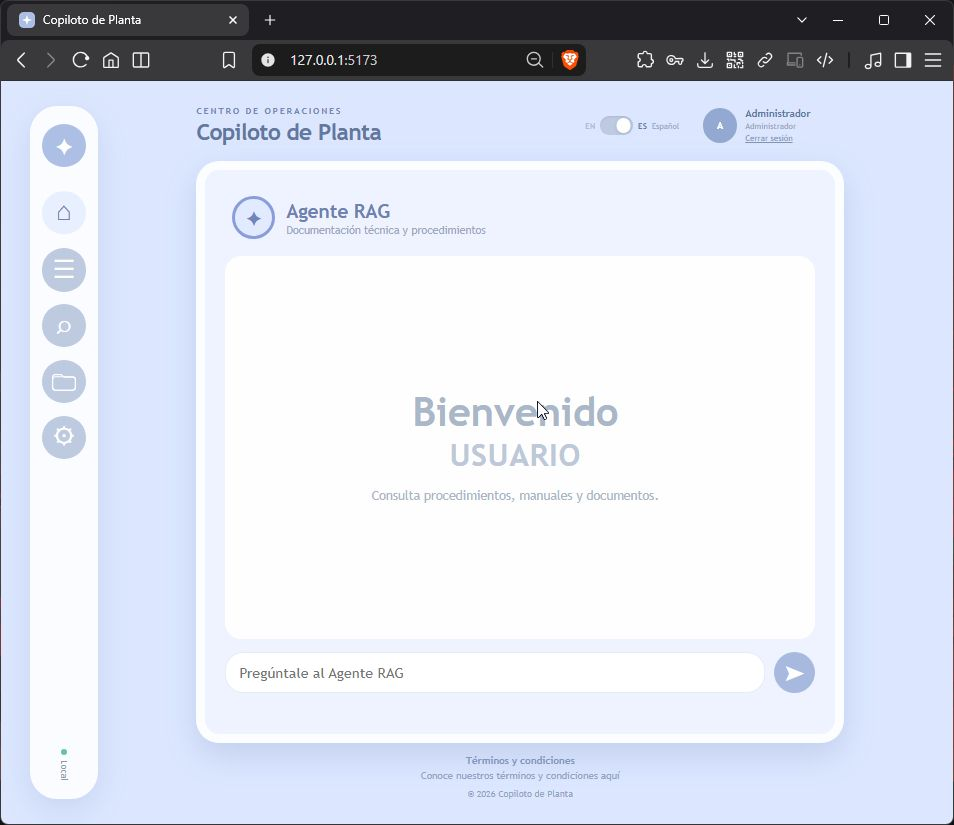
\includegraphics[width=0.48\textwidth]{img/pantalla_inicio.png}
\caption{Pantalla inicial del copiloto web.}
\label{fig:pantalla_inicio}
\end{figure}

La Figura~\ref{fig:pantalla_chat} muestra una consulta respondida a partir de los documentos indexados. La interfaz
presenta la pregunta, la respuesta en formato legible, el estado de recepción y enlaces a las fuentes. Esta pantalla
atiende los casos de uso de consultar documentación, recuperar fragmentos y abrir una fuente. La respuesta de prueba
identifica la presión nominal de la prensa PH-100 y su tolerancia; los datos fueron tomados del corpus local y no se
introdujeron credenciales ni información confidencial.

\begin{figure}[H]
\centering
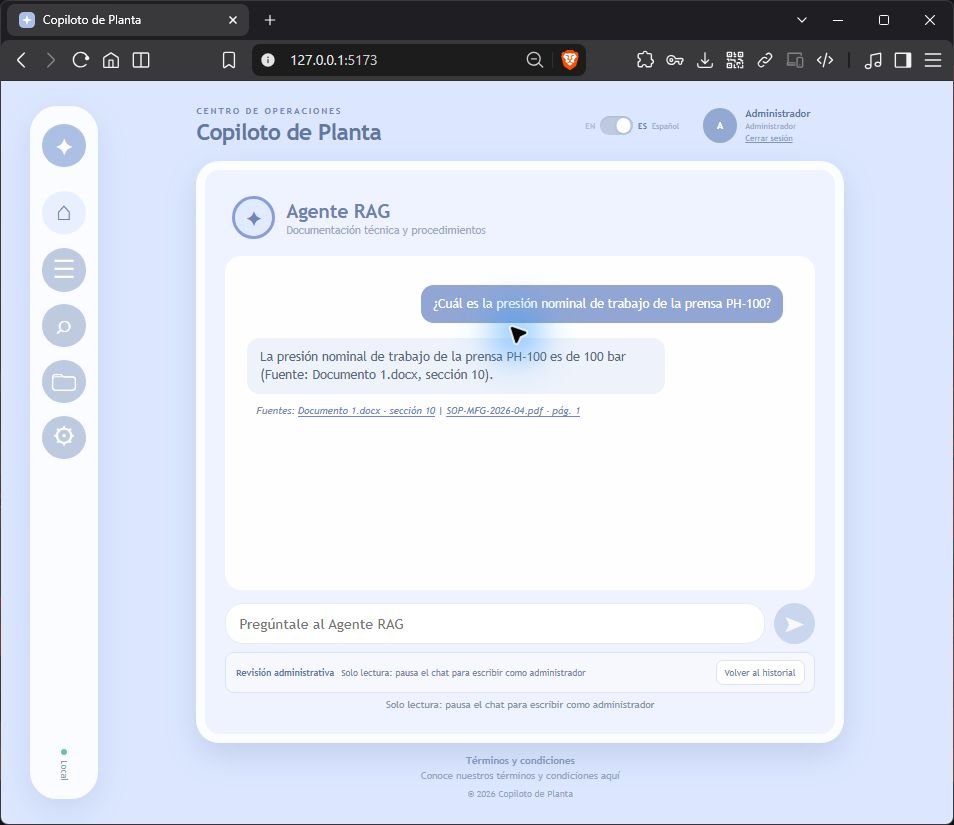
\includegraphics[width=0.48\textwidth]{img/pantalla_chat_respuesta.png}
\caption{Respuesta del agente con fuentes documentales.}
\label{fig:pantalla_chat}
\end{figure}

La pantalla de historial permite continuar una conversación sin perder sus mensajes. En la Figura~\ref{fig:pantalla_historial}
el título corresponde a la primera pregunta y se muestra una vista previa, el número de mensajes y la fecha de actualización.
El usuario puede abrir el chat para revisar el contexto anterior o iniciar uno nuevo. La sesión del navegador se utiliza para
separar los chats de prueba y el backend verifica que el identificador solicitado pertenezca a esa sesión.

\begin{figure}[H]
\centering
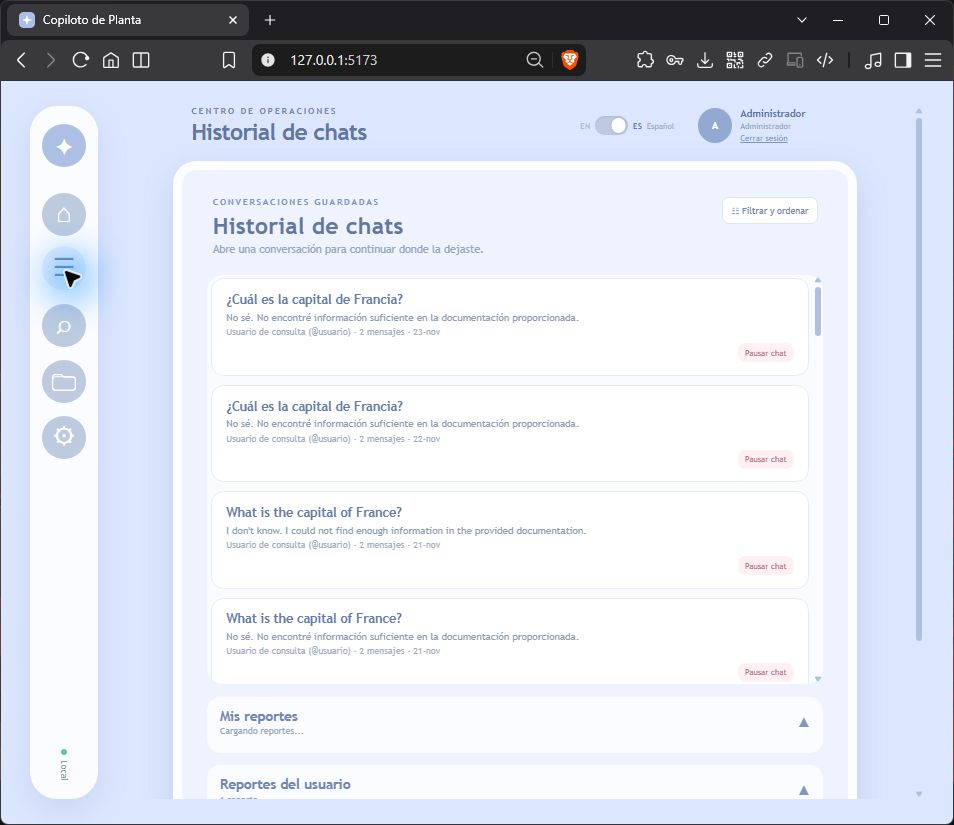
\includegraphics[width=0.48\textwidth]{img/pantalla_historial.png}
\caption{Historial de conversaciones del usuario de prueba.}
\label{fig:pantalla_historial}
\end{figure}

La biblioteca de documentos atiende al responsable documental y permite comprobar qué archivos están disponibles. La
Figura~\ref{fig:pantalla_documentos} muestra seis documentos de prueba clasificados por extensión, un buscador y el botón
para subir archivos permitidos. La carga valida extensiones y tamaño máximo en la API; además, el sistema advierte que
subir un archivo no sustituye el proceso de extracción, fragmentación e indexación. Así se distingue la administración de
archivos de la preparación del corpus que utiliza el agente.

\begin{figure}[H]
\centering
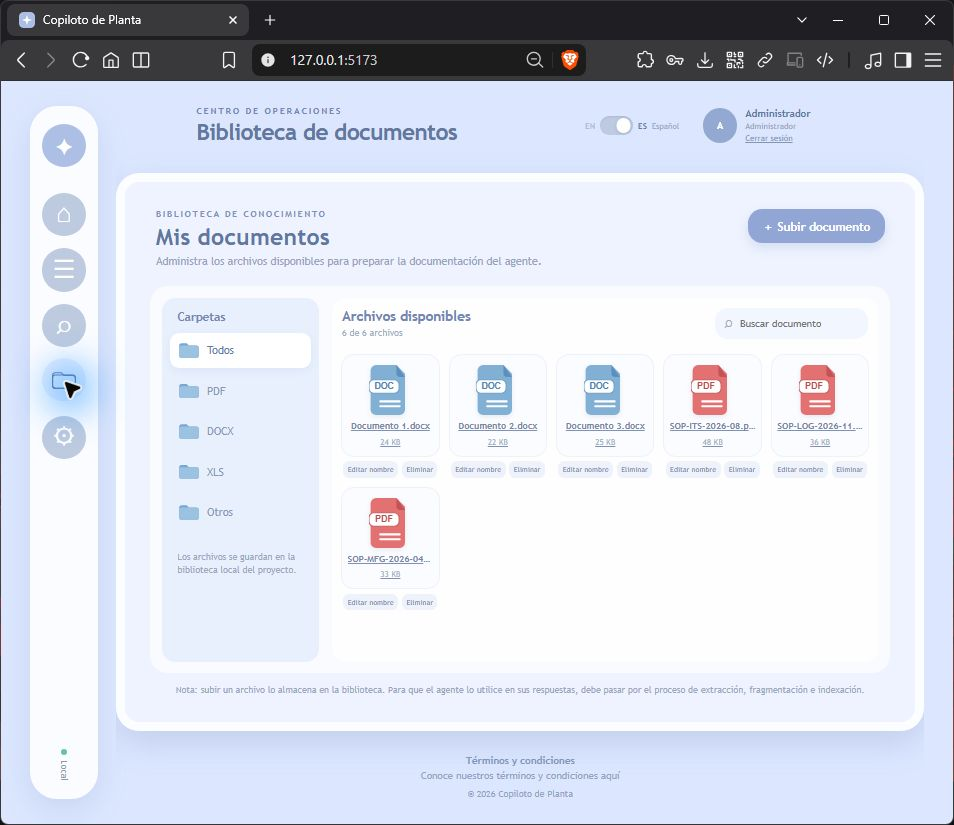
\includegraphics[width=0.48\textwidth]{img/pantalla_documentos.png}
\caption{Biblioteca local de documentos técnicos.}
\label{fig:pantalla_documentos}
\end{figure}

En conjunto, las pantallas cubren el flujo visible del prototipo: iniciar una consulta, recibir una respuesta trazable,
continuar un chat y revisar los documentos disponibles. La evidencia visual corresponde a una ejecución local comprobada
con el backend activo y complementa los diagramas de arquitectura, casos de uso, actividades y secuencia.
